\documentclass[conference,a4paper,10pt,oneside,final]{tfmpd}

\usepackage[spanish]{babel}
\usepackage[utf8]{inputenc}
\usepackage{graphicx}           % inserción de graficos

\begin{document}

	\title{Interfaz aérea}
	\author{Bedrij Walter, Benitez Federico y Benitez Fernando \\
	\textit{Trabajo práctico final de ``Procesamiento digital de imágenes'', II-FICH-UNL.}}
	\markboth{PROCESAMIENTO DIGITAL DE IMÁGENES: TRABAJO FINAL}{}
	\date{}

	\maketitle

\begin{abstract}
	En el desarrollo de las interfaces aéreas suelen utilizarse marcadores, 
	cuya forma y color sean fácilmente identificables, o dispositivos 
	de captura y emisión por fuera del rango de la luz visible.
	El trabajo presenta un método que presenta menores restricciones para el usuario, al no utilizar marcadores y teniendo una webcam como dispositivo de captura. 
	Se analizan distintas características que permitan la detección de la posición de las manos, preocupándose de que éstas sean robustas ante distintas condiciones de iluminación y transformaciones de escalado y rotación, pero que puedan ser implementadas en tiempo real.
	Los errores de localización son tratados mediante un sistema predictor-corrector (filtro de Kalman), suavizando la trayectoria. 
\end{abstract}
	\begin{keywords}
   		 Interfaz aérea, segmentación, markless, filtro de Kalman
	\end{keywords}

    \section{Introducción}
	El objetivo del trabajo desarrollar un algoritmo que permita localizar la posición de las manos y describir su trayectoria teniendo como entrada un vídeo sacado de una cámara web.
	Siendo luego aplicado a la creación de interfaces aéreas sin la utilización de marcadores.

	El trabajo no aborda el seguimiento de la mano, simplemente se trata a cada fotograma de manera independiente. 
No supone mayor penalidad en  el tiempo de ejecución, 
sin embargo imposibilita la resolución de casos en donde
la mano se encuentra sobre la cara.

Además se supone que el brazo se encuentra cubierto. 
Si bien la detección sería mucho más simple (al menos en el caso de que no exista superposición), se dificulta la elección de un punto característico.

   	 El procesamiento es como sigue:
   	 \begin{enumerate}
   		 \item Obtención de una imagen de referencia para el fondo
   		 \item Captura de los fotogramas del vídeo
   		 \item Diferenciación con el fondo
   		 \item Enmascaramiento de la piel
   		 \item Identificación de las manos (eliminación de la cara)
   		 \item Ubicación del puntero
   	 \end{enumerate}

    \section{Materiales y métodos}
   	 \subsection{Obtención de una imagen de referencia}
		Con el objeto de eliminar objetos estáticos del análisis, 
   		 permitiendo así que la mano se sitúe en zonas de coloración parecida
   		 sin mayores problemas, 
se procede a la captura de la imagen del fondo.
		
		La cámara elegida realiza un ajuste automático, esto supone inconvenientes ya que el fondo con y sin objetos resultarán distintos a pesar 
	de que las otras condiciones (como la iluminación) permanezcan constantes.

   		 Con respecto a la iluminación, esta se considera constante e incidente,
   		 evitando una excesiva potencia que pudiera lavar los colores.

   	 \subsection{Captura de los fotogramas del vídeo}
   		 Cada fotograma es tratado de manera independiente.
   		 Se adquiere una imagen a color, y se la separa en los canales HSV.
		
		Los frames se envían a los procesos de diferenciación con el fondo 
		y de segmentación de la piel.

En cuanto a la posición de los objetos, se espera que las manos y la cara se encuentren completamente dentro del fotograma y que no se superpongan.

   	 \subsection{Diferenciación con el fondo}
		Se realiza la diferencia entre los canales RGB del frame actual contra
		la imagen de referencia del fondo.
		Esto permite discriminar al objeto.

   	 \subsection{Enmascaramiento de la piel}
   		 En esta etapa se analizaron parámetros que pudieran hacer
   		 más factible la separación del objeto de interés.
   		 Como ser el hue, la saturación, la intensidad, y combinaciones entre las mismas
   		 
   		 Se observó que la saturación era muy dependiente de la iluminación, por lo que fue descartada.
   		 En el caso de la intensidad cambios en la posición del objeto creaban sombras y reflexiones que impedían fijar un umbral.
   		 Sin embargo, el hue era un parámetro robusto ante distintas intensidades de iluminación.
		
		Fue posible ajustar un umbral global donde no se prestara a una confusión visual de fondo-figura.
		Sin embargo, dada las características de la piel, no se lograba atrapar a una gran cantidad de píxeles de interés. 
Afortunadamente, no conformaban aglomeraciones, sino que se hallaban distribuidos (observándose un efecto de puntillado en la máscara), 
por lo que pudieron recuperarse mediante una dilatación.

Algunos objetos del fondo que fueron capturados pudieron ser eliminados realizando la diferencia con la imagen de referencia. 
   		 
   		 También se analizaron con combinaciones lógicas entre los canales, pero debido a las desventajas ya nombradas
   		 no se tuvo mayor éxito que hue solo.

		Se decidió ocupar solamente la información del hue.
		Como preproceso se aplica un filtro de mediana, tratando además de uniformar la textura de la piel.
   		 %Se aplica un filtro de mediana para eliminar el ruido impulsivo en el hue.
	%no es ruido impulsivo, son las venas (azul)
   		 Se realiza un umbralizado global en el hue dejando pasar el rango $H = 7 \pm 5$ (valores experimentales de la piel)

   		 Para eliminar los huecos internos en el hue, se procedió aplicar una dilatación con una máscara de $5 \times 5$,esto provoco un grado de deformación
   		 en los objetos, luego para recuperar medianamente la forma original, se procedió a una erosión con máscara también de $5 \times 5$

   		 Se combina con la máscara de diferencia, obteniéndose entonces
   		 objetos no pertenecientes al fondo con un tono parecido al de la piel.

   		 \subsubsection{Crecimiento inverso de regiones}
			Otro método para eliminar los huecos dentro de las regiones es el crecimiento inverso.
   	
			Trabajando sobre la máscara binaria del hue,		 
   			 a partir de un punto que se conoce fuera de cualquier zona de interés,
			realizamos el crecimiento de regiones. Con esto obtenemos el fondo, 
			al invertir la máscara se tendrán las siluetas de los objetos.


    \subsection{Eliminación de la cara}
   		 Luego del proceso anterior, se tiene una imagen compuesta por objetos
   	 tipo piel. Estas pueden ser la cara, las manos y algún ruido que haya pasado los filtros.

   		 Por eso se etiquetan las regiones, quedándose con las $3$ de mayor área,
   	 que se supone pertenecientes a ambas manos y la cara.
   	 Por observación debieran de tener un área similar, si resulta que alguna
   		 es excesivamente pequeña con respecto a las otras ($25\%$) es considerada
   	 como ruido y eliminada.

   	 
   		 Queda discriminar las correspondientes a las manos,
   	 es decir, eliminar la región que identifica a la cara.

   	 Para facilitar el proceso, la mano debe tener un dedo extendido.
   	 Suponiendo a la cara como redonda, es de esperar que al hacer
   	 el coeficiente
   		 \[C = \frac{\mbox{Área}}{\pi r^2}\]
   	 este sea cercano a $1$. Donde $r$ es el radio del círculo cuyo centro
   	 se corresponde al centroide de la región y pasa por su punto más alejado.

    \subsection{Ubicación del puntero}
   	Al finalizar el proceso anterior se tienen las áreas interesantes.

   	 Se ubica al puntero como al punto más lejano del centroide de la región.
 Para suavizar la trayectoria del puntero, se utiliza un modelo predictor-corrector, en este caso aplicando un filtro de Kalman.
Se pueden observa que los punteros son independientes, es decir que el usuario puede sacar de escena  una de las dos manos.

\subsection{Diseño de interfaz}
  Para implementación de la interfaz se diseño una paleta de colores que consiste en 5 colores : rojo, verde, azul, blanco y negro. También se diseñaron dos objetos, el borrador y el visor de color actual.

La manipulación consiste en tener el dedo índice bien extendido, el dedo índice izquierdo se utiliza para la selección del color y del borrador, el dedo índice derecho es el puntero para dibujar.

	
\section{Resultados}
		El uso de una imagen de referencia para el fondo permitió que la mano se ubicara sobre zonas de tonalidad parecida.
		Sin embargo, la cámara utilizada tenía función de auto-foco, por lo que se creaban falsas diferencias. 

Una de las aproximaciones para tratar este problema fue la de comparar contra la imagen anterior, pero se desechó rápidamente al notar que podrían surgir nuevas regiones al ocultar y descubrir el fondo.
Se optó finalmente por incrementar el umbral de la diferencia, dejándolo en $30/255$

		El hue mostró ser bastante robusto a los cambios de intensidad de iluminación, por lo que pudo fijarse un umbral en forma experimental y no se necesitaba de una posterior calibración. 
Éste fue probado con dos tipos de piel, usando iluminación por lámpara incandescente y fluorescente (compacta).
		%Sin embargo, se tuvo problemas con el ajuste de blancos de la cámara,
		%tomando la piel clara una tonalidad azulada en vez de rojiza al usar lámparas incandescentes. (discutir)

	La lámpara incandescente producía artefactos en el hue, detectándose como válida la zona de mayor intensidad. Una alternativa podría ser la de difuminarla antes.
	
	En la detección de la mano, el mayor problema lo presenta un enmascaramiento defectuoso, sobre todo al generarse sombras por la propia posición de la mano.

En caso de que el dedo se considerara como una región separada seria eliminado por su área insignificante, quedando solo la palma
de forma aproximadamente circular, por lo que la heurística fallaba.
	% que fede tire algo después por acá
	La heurística permite independencia de la escala, pudiendo entonces usar la interfaz tanto de forma cercana (sentado frente a la pc) como a distancia ($1m) %probar

	Sin embargo, se requiere la presencia de ambas manos y de la cara en los fotogramas. Es posible detectar el caso de una sola mano, pero los ruidos pueden cobrar importancia y presentar falsos positivos

		Con respecto a la interfaz observamos unas oscilaciones instantáneas producto de detecciones de puntos lejanos no deseados con respecto al centroide de las manos como en el caso cuando se usa la interfaz con una remera corta, como este método se basa en diferencias de imágenes y hue, el brazo sobrevive a los procesamientos  de eliminación, y como es aproximadamente del mismo color de la mano, es segmentado obteniendo así puntos lejanos no deseados, por ello una de las restricciones es usar  atuendo que oculte el brazo y descubra las manos.

		A través del predictor-corrector se pudieron reducir las oscilaciones del puntero, 
	sin embargo el tiempo de respuesta se vio afectado. 
	Se tiene un compromiso entonces entre velocidad y precisión, en caso de que la segmentación de la mano
	presente problemas sería útil utilizar Kalman.

	\section{Conclusión y trabajos futuros}
		La detección de la posición de las manos fue posible en tiempo real,
		si bien se usaron suposiciones como que los brazos estuvieran cubiertos
		y de que no ocurriera superposición.

		Los criterios de discriminación de las manos obligó a 
		usar una conformación en las posiciones de los dedos. 

		Problemas en la segmentación generaba falsas identificaciones, 
		lo que se traducía en discontinuidades en las posiciones de los punteros.

		Para intentar solventar esos problemas, se propone realizar tracking
		de las manos, requiriendo simplemente una detección global inicial.

		Se puede realizar un refinamiento en la selección del punto característico
		correspondiente a las manos. Por ejemplo, poder discriminar los dedos
	\section{Figuras}

	\begin{figure}[tbhp]
	\centerline{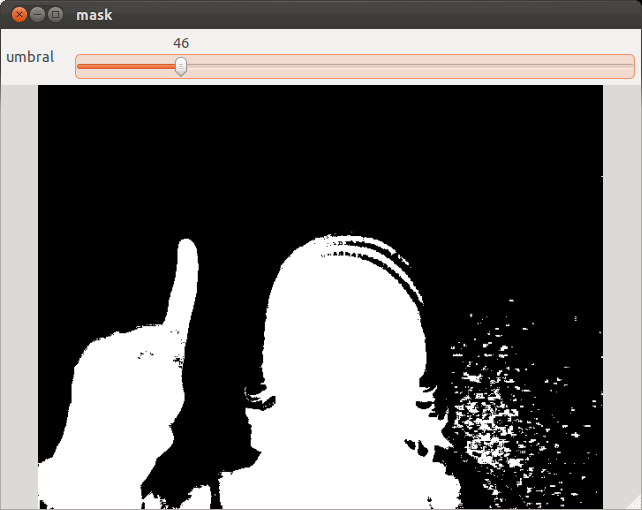
\includegraphics[scale=0.2]{3_mask}}
	\caption{Diferencia contra el fondo de referencia}
	\label{fig:diferenciacion}
	\end{figure}
	

	\begin{figure}[tbhp]
	\centerline{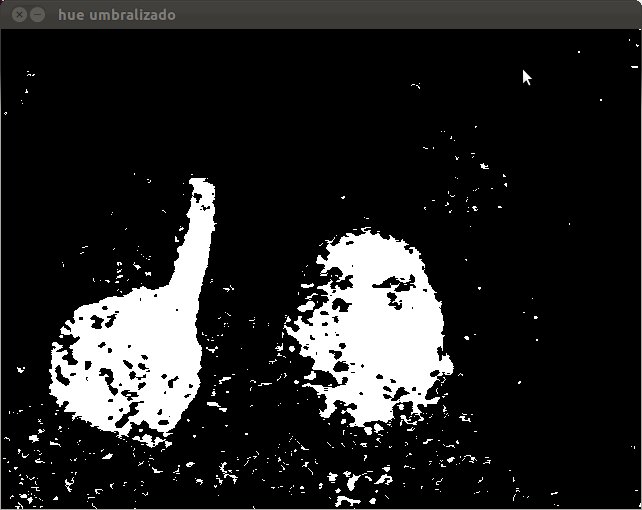
\includegraphics[scale=0.2]{2_hue_umbralizado}}
	\caption{Umbralizado del hue}
	\label{fig:hue_umbral}
	\end{figure}
	
	\begin{figure}[tbhp]
	\centerline{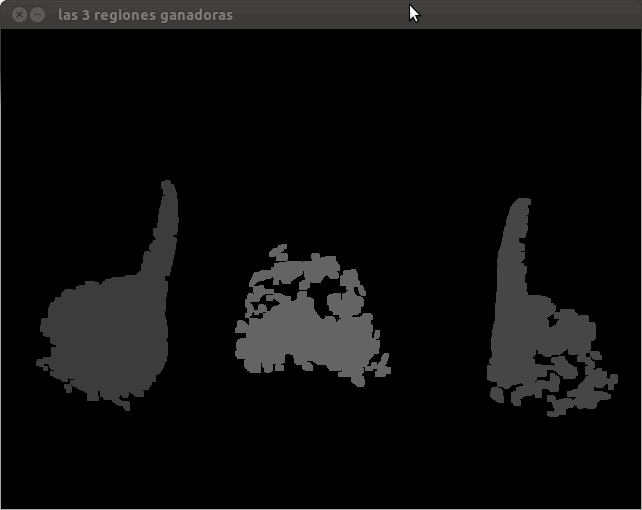
\includegraphics[scale=0.2]{5_3_regiones_ganadoras}}
	\caption{Regiones ganadoras}
	\label{fig:ganadoras}
	\end{figure}
	
	
	\begin{figure}[tbhp]
	\centerline{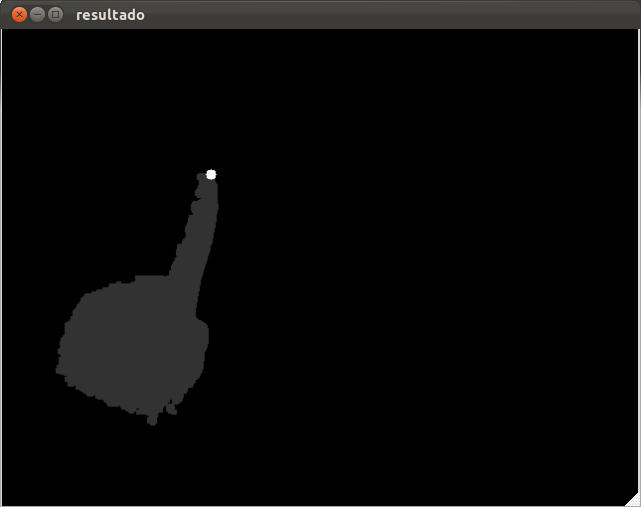
\includegraphics[scale=0.2]{6_resultado_final}}
	\caption{Casos}
	\label{fig:casos}
	\end{figure}
	
	\begin{figure}[tbhp]
	\centerline{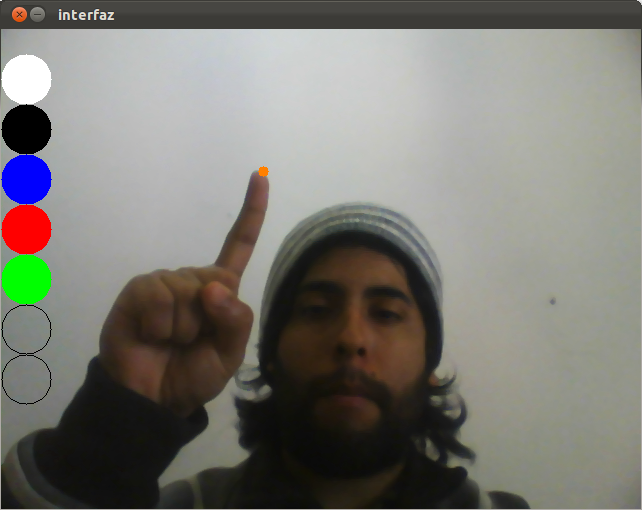
\includegraphics[scale=0.2]{7_interfaz}}
	\caption{Interfaz}
	\label{fig:7_interfaz}
	\end{figure}
	
	
	\nocite{*}
	\bibliographystyle{tfmpd}
	\bibliography{interfaz_aerea}


\end{document}

